\section{Entrepreneurial Education (EE)}
\label{sec:EE}

\begin{itemize}
\item Henry 2005 - Can entrepreneurship be taught? (maybe nice for introduction)
\item  Kuratko, Donald F. (2005): The Emergence of Entrepreneurship Education. Development, Trends, and Challenges 
\end{itemize}

\subsection{Categories of EE Courses/Approaches (Theory)}
Do such categories exist? (i.e. practical - theoretical; tech - biz; ...)
\begin{itemize}
\item Pittaway 2007 - Literature review: general positive impact of EEP on EI and propensity, but rarely quantified; also: do people become better entrepreneurs after courses? Points out that there is no clear understanding of enrepreneurship education:
see summary later
\item Loi 2015 - The theoretical foundations of entrepreneurship education: How co-citations are shaping the field (maybe not well suited for this):
\begin{itemize}
\item 
\end{itemize}
\item Garavan 1994 - Entrepreneurship Education and Training Programmes: A Review and Evaluation (hope it helps here)
\item (new) Kuratko 2005 - The Emergence of Entrepreneurship Education: Development, Trends, and Challenges
\item (new) Laukkanen 2000 - Exploring alternative approaches in high-level entrepreneurship education: creating micro- mechanisms for endogenous regional growth (maybe too much focus on economy)
\item (new - but no paper) Plaschka 1990: Emerging Structures in Entrepreneurship Education: Curricular Designs and Strategies
\end{itemize}

\begin{figure}[h]
\begin{center}
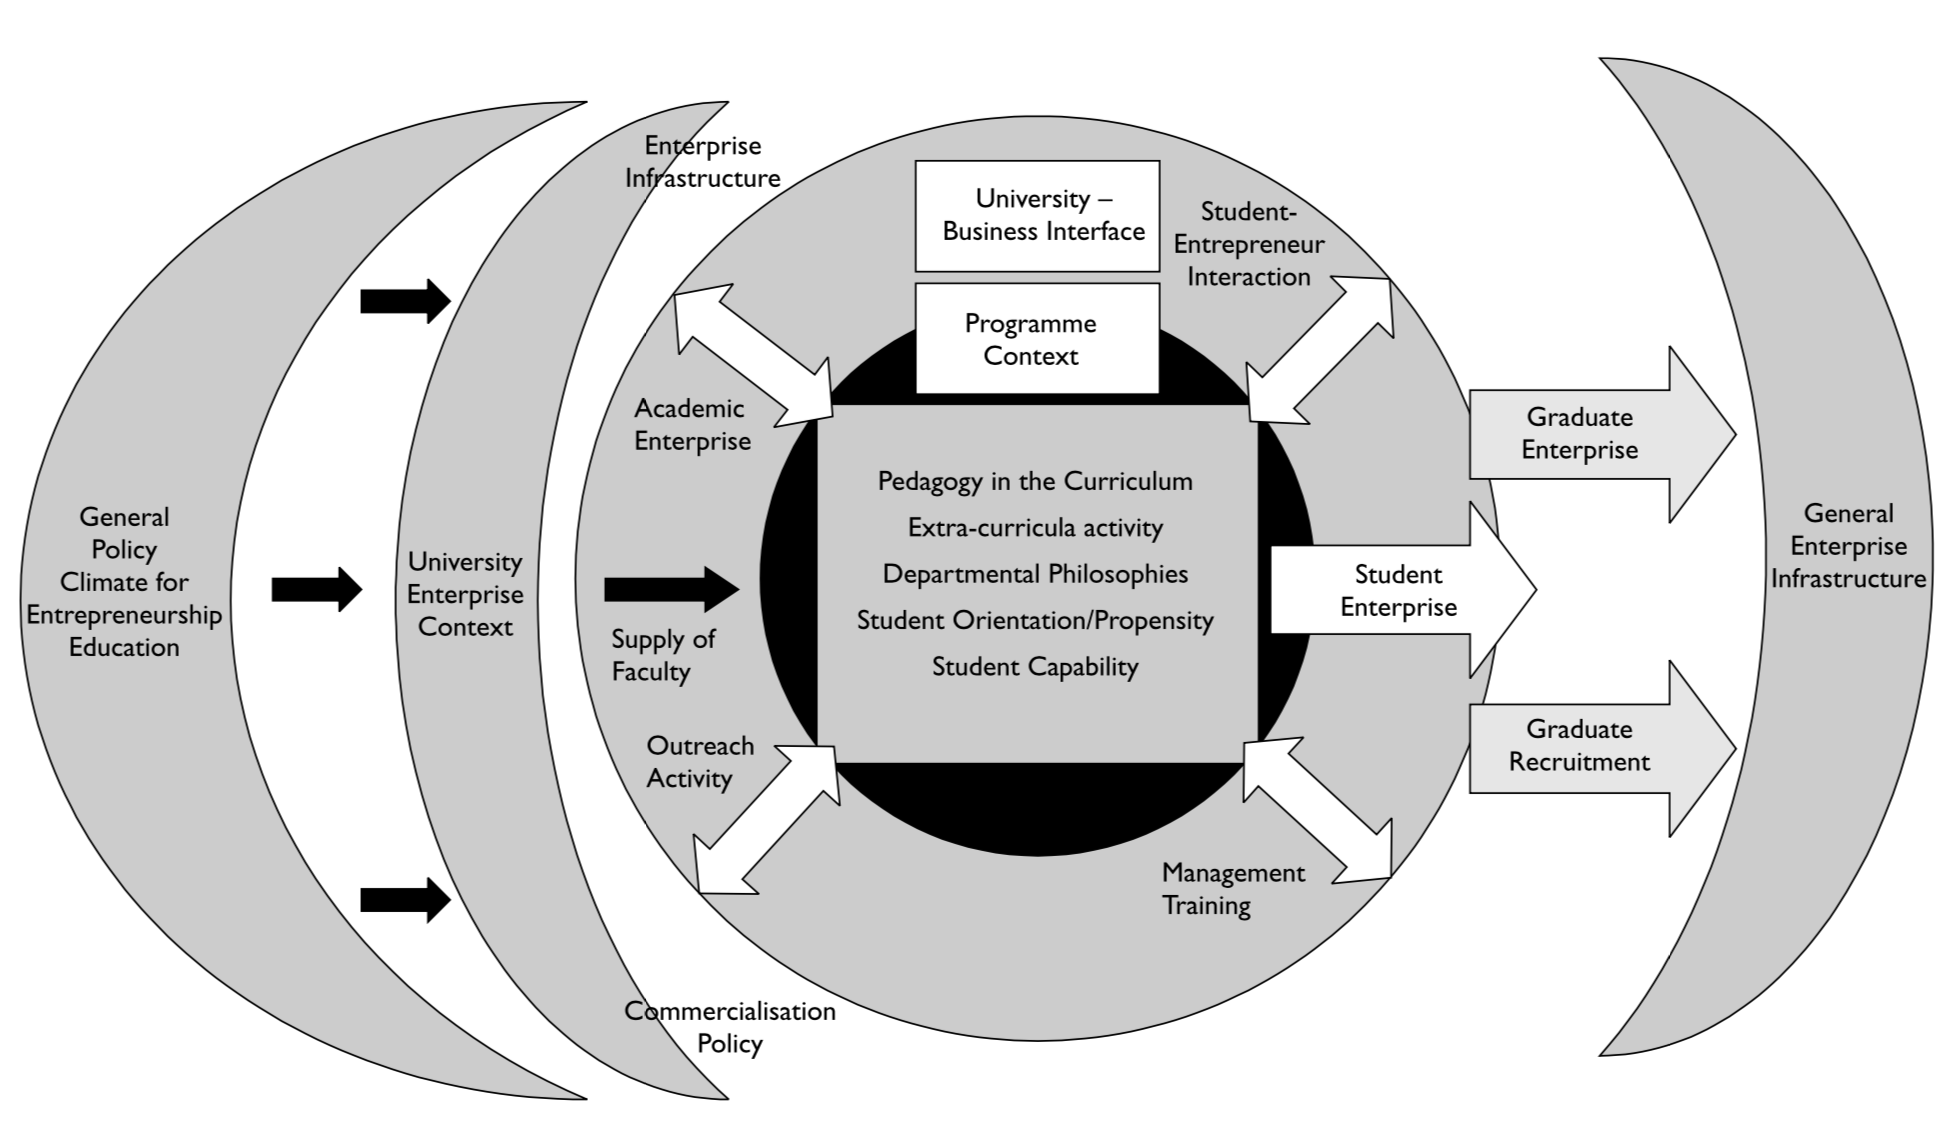
\includegraphics[width=\textwidth]{images/framework-EE}
\caption{A Thematic Framework for Entrepreneurship Education}
\label{fig:framework-EE}
\end{center}
\end{figure}

\subsection{How EE courses can be assessed (Theory)}
Suggested Literature:\\
\begin{itemize}
\item Fayolle 2006 (proclaimed new approach of assessing EEPs)
\end{itemize}

\subsection{Previous Findings about EE impact on intentions (literature)}
Suggested Literature
\begin{itemize}
\item Fayolle 2015 - Study of long term impact of EEP on EI, also under considerations of previous exposure to entrepreneurship. Little previous exposure: positive impact of EEP on EI, high previous exposure: negative impact of EEP
\begin{itemize}
\item "we propose an original research design where (1) we measure the initial state and persistence of the impact and not only short-term effects; (2) we deal with a compulsory program, allowing to avoid self-selection biases; and \textbf{(3) we deal with an homogeneous "compact" program rather than programs combining multiple teaching compo- nents whose effects cannot be disentangled"}
\item main research results show that the positive effects of an EEP are all the more marked when previous entrepreneurial exposure has been weak or inexistent. Conversely, for those students who had previously significantly been exposed to entre- preneurship, the results highlight significant countereffects of the EEP on those participants.
\item researchers and institutions interested in studying effect
\item experiemnt meausres  impact of a short and compulsory entrepreneurship education program (EEP) + factors (predispo- sitions, time) influencing this impact
\item Zhao, Hills, and Seibert (2005) underline a gap in the literature + need to evaluate the effectiveness of different types of entrepreneurship programs depending on their key components (content, design, and delivery). 
\item found: only effect on students without contact to entrepreneurship, but then persistence of this impact six months after the program.
\item main theoretical contribution: confirm that intention models, (theory of planned behavior) may be diverted from their initial objective (a predictor of the behavior) in order to be used as indicators of the impact of EEPs + \textbf{suggest that such intention models should attribute greater importance to factors related to previous entrepreneurial exposure}
\item "practical point of view, this paper provides concrete perspectives and directions regarding the elaboration, design, and orientation of EEPs, in a time of strong demand for such programs."
\item theoretical framework is based on the theory of planned behavior and adds as key variables the initial level of intention and the prior entrepreneurial exposure.
\end{itemize}
\item Lorz 2011 - Insignificant or even negative impact of EEP on EI
\begin{itemize}
\item dissertation of 140 pages :O
\item quantitative and a qualitative section
\item "For the quantitative section, a quasi-experimental, ex-ante/ex-post, control group, longitudinal (up to 18 months), repeated measures research design was implemented, with a total of 272 matched pairs (Tstart/Tfinal)" (theory of planned behaviour was utilised as the underlying theoretical mode)
\item qualitative part of the study, a content analysis of 55 reflection papers was conducted.
\item \textbf{"results attest to an insignificant impact of entrepreneurship education on entrepreneurial intention"}
\item insignificant impact was not moderated by the length of an entrepreneurship education
\item \textbf{"An analysis of the development of entrepreneurial intention after the end of an entrepreneurship programme showed that after six months entrepreneurial intentions had decreased significantly. Entrepreneurship education is confirmed to be a major source of inspirational triggers that positively impact on entrepreneurial intention."}
\item Research has, to date, contributed to this belief and underlined the positive impact of entrepreneurship education (Chrisman, 1997; Peterman + Kennedy, 2003; Zhao, Seibert, + Hills, 2005).
\item "Out of 41 studies analysing the impact of entrepreneurship education, 39 indicated a positive or mixed result (Lorz, Müller, + Volery, 2011)."
\item "Only recently did two studies find a negative impact of entrepreneurship education (Oosterbeek, van Praag, + Ijsselstein, 2010; von Graevenitz, Harhoff (der ist LMU prof), + Weber, 2010). At second glance, it appeared that most studies that had reported a positive impact of entrepreneurship education had significant methodological deficiencies, which strongly limited the validity of the results."
\item all paper with positive effects had significant methodological deficiencies: didn't measure direct impact, used no control group, small samples, mixed results
\item provides table comparison (see: \ref{fig:table-negative-impact})
\item RQ: What impact does an entrepreneurship education programme have on entrepreneurial intention?, hat is the impact of the duration of an entrepreneurship programme on entrepreneurial intention and its antecedents?
\item new variants of entrepreneurship education programmes are tested with respect to their impact
\end{itemize}

\item Martin 2013 - Effect of EET on human capital formation, positive impact of EET on entrepreneurship, though, overestimated by previous studies due to methodological weaknesses
\begin{itemize}
\item 
\end{itemize}

\item Oosterbeek 2010 - insignificant impact of EEP on entrepreneurial skill, negative impact on intent

\item Pittaway 2007 - Literature review: general positive impact of EEP on EI and propensity, but rarely quantified; also: do people become better entrepreneurs after courses? Points out that there is no clear understanding of enrepreneurship education
\begin{itemize}
\item "The findings support the conclusion that entrepreneurship education has had an impact on student propensity and intentionality"
\item "unclear is the extent
to which such education impacts on the level of graduate entrepreneurship or whether it enables graduates to become more effective entrepreneurs"
\item "lack of consensus on what entrepreneurship or enterprise education actually is " in practice
\item table about thematic coding of literature review
\item thematic framework highlighting conceptual key areas for empirical research in entrepreneurship education (see figure \ref{fig:framework-EE})
\item Each element explained in paper (a lot of blabla)
\item lists research gaps: longitudinally graduate careers; graduate entrepreneurship and recruitment or demand from employers; \textbf{"Although there is study that has linked entrepreneurship education to out- comes like graduate venture creation the area has been under researched overall"}, supranational policy
\end{itemize}
\item Sanchez 2013: Positive impact of EE on intenation AND competencies(!!!) (compare with Oosterbeek 2010). Also: contribution to TPB
\item Solesvik 2013: plain test of impact of EE on EI according to TPB (looks pretty boring)

\item Zhao 2005 - Effects of Perceived Learning from EE, Preveious E-Experience and risk propensity on EI are fully mediated by entrepreneurial self-efficacy

\item For the end of this chapter: Lorz 2013 - methodological insufficiencies of studies about EEP on EI. According to the paper, most studies show positive impact, but this paper doubts it. How to improve studies. (Kevin: be careful, if we have not implemented the recommendations of the study)
\end{itemize}


\begin{figure}[h]
\begin{center}
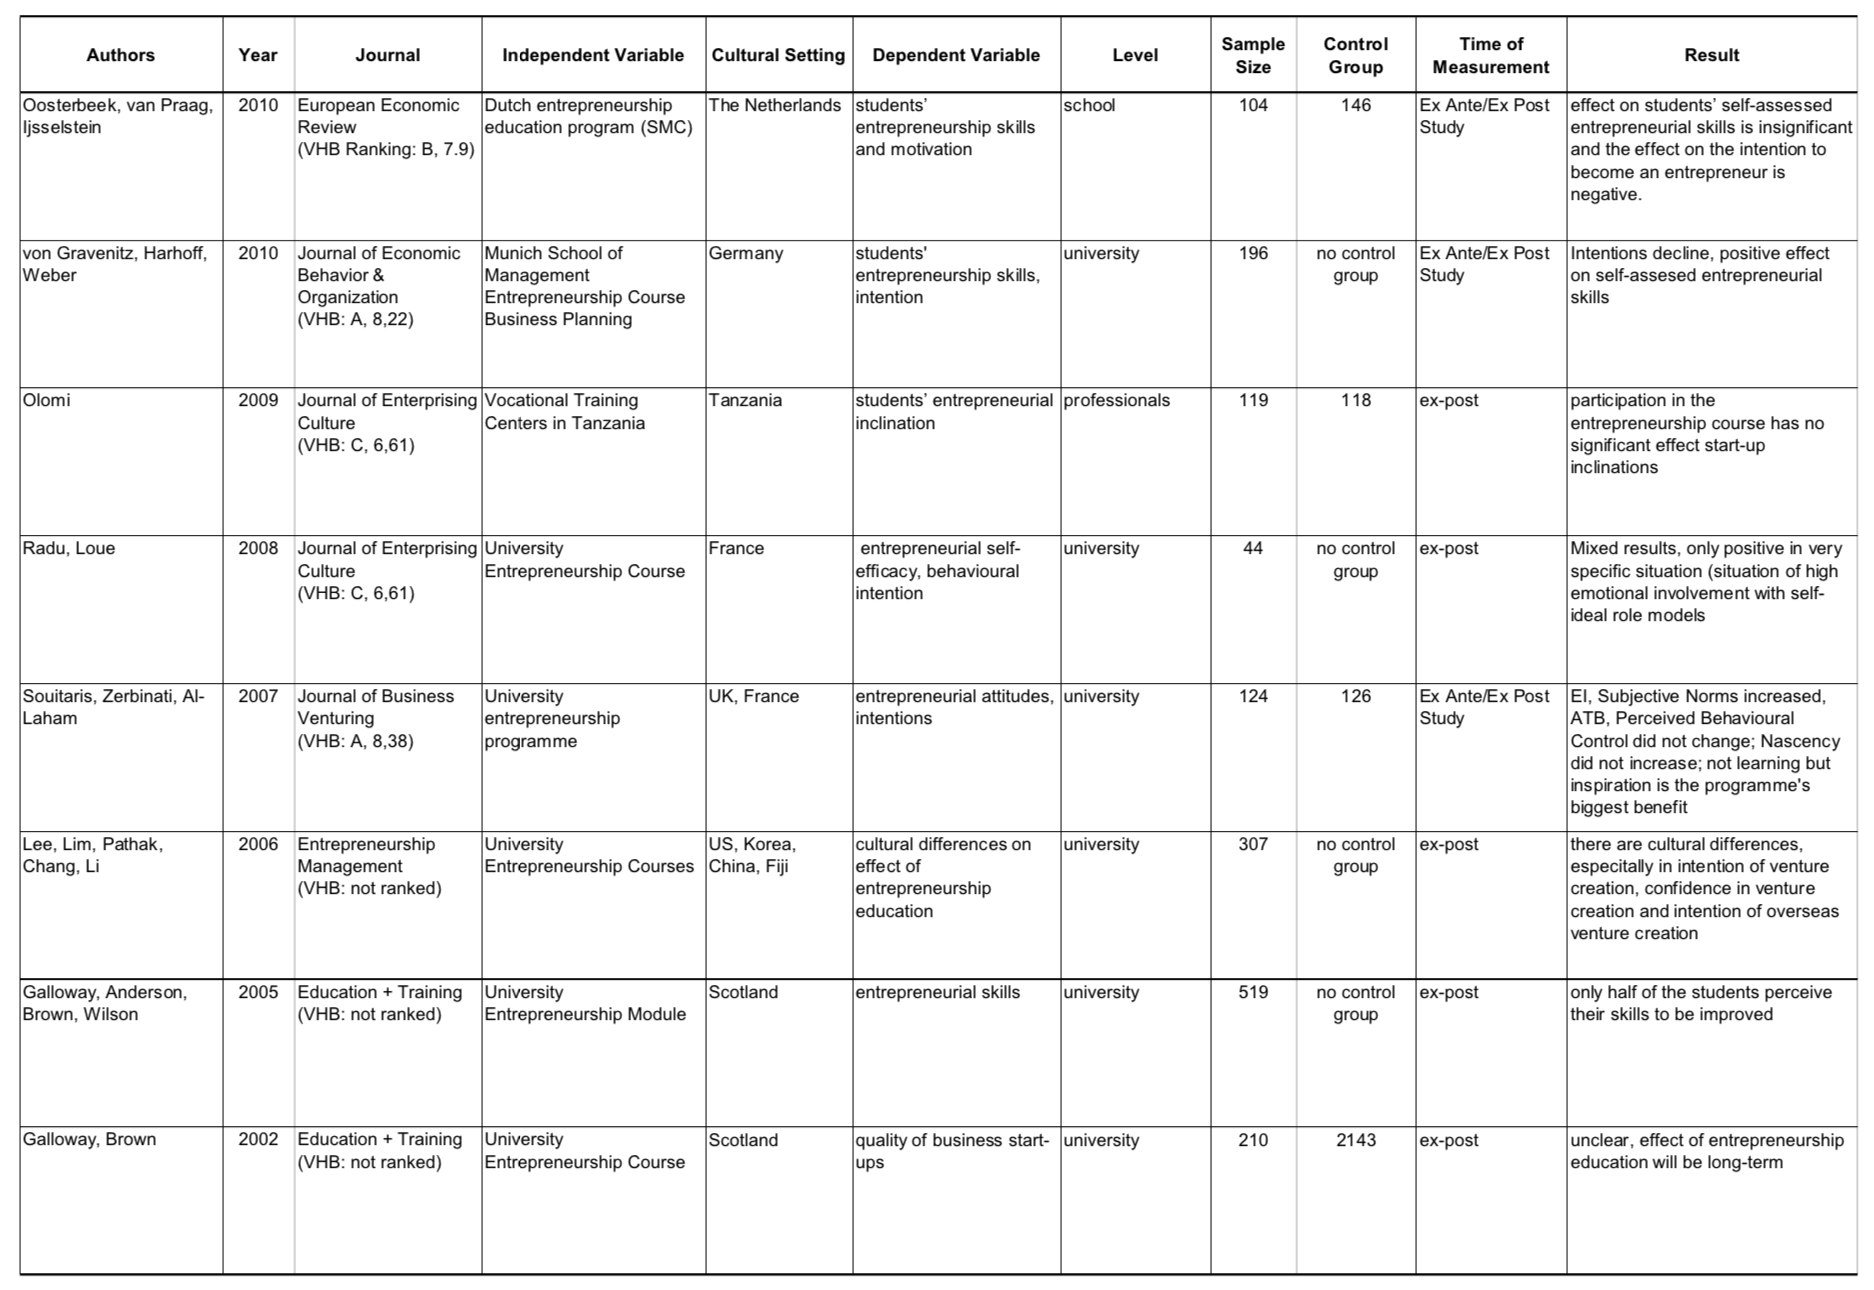
\includegraphics[width=\textwidth]{images/table-negative-impact}
\caption{Overview of Negative and Insignificant Studies}
\label{fig:table-negative-impact}
\end{center}
\end{figure}

\subsubsection{Structure of the EEP (tech. prototyping, business plan, design thinking, etc.)}

\subsubsection{Setting of the study (Training vs. education focused)}

\begin{itemize}
\item Lourenco 2016 - Developing Entrepreneurship Education: Comparing Traditional and Alternative Teaching Approaches (maybe a C or D Paper)
\end{itemize}

\subsubsection{Background of study subjects (technical, business, etc.)}

\begin{itemize}
\item Souitaris 2007 - Impact of EEP on EI among tech students; TPB; EEP positively influence emotions towards entrepreneurship
\item Maresh 2016 - EE impact comparison on tech and biz students
\end{itemize}

\subsubsection{Mandatory classes - from here we can derive the research gap again}
\begin{itemize}
\item von Graevenitz 2009: Study of MANDATORY EEP on EI; negative impact on intentions, positive impact on self-assessed skills
\end{itemize}